\documentclass[12pt]{IEEEtran}
\usepackage{graphicx}

\author{Ralph Krimmel}
\title{An overview of current BGP security problems}


\begin{document}
	\maketitle
	\begin{abstract}
	\end{abstract}
	\section{Introduction}
	Communication in today's internet is possible by the interplay of many protocols. 
	On the so called internet layer the Internet Protocol \emph{IP} is the primary protocol that is used to forward network packets (datagrams) to the respective target hosts or network. 
	IP networks are grouped as autonomous systems or in short \emph{AS}, networks under control of one organization. 
	The relaying of those packets inside or between networks is done by every host that speaks IP, but most importantly by special hosts, called routers. 
	A router has to decide which will be the next hop the datagram has to be moved to. 
	This can either be inside or between autonomous systems. 
	To perform this decision, routers make use of additional protocols which are classified as \emph{intradomain routing protocols} for routing in, and \emph{interdomain routing protocols} for routing between ASes. 

	The prevalent interdomain routing protocol is BGP, the \emph{Border Gateway Protocol}, or more specific \emph{Exterior Border Gateway Protocol}. 
	In practise BGP works basically well but the lack of security mechanisms and performance guarantees makes it vulnerable against attacks or configuration mistakes. 
	There have been a few incidents in the past where misconfigured routers reduced the functionality of bigger parts of the internet. 
	With manipulated BGP messages, even more harm could be caused if those messages are intelligently sent to specific and important targets. 
	Therefore it is still highly important to research methods to make BGP secure, performant and reliable. 

	\section{The Border Gateway Protocol}
	The Border gateway protocol is an incremental protocol that enables border routers of adjacent autonomous systems to exchange information on how to reach blocks of IP adresses or so called \emph{IP prefixes}. 
	Incremental means, that BGP transfers changes of routes and not complete routing tables in every message.

	Another important information that is contained in specific BGP messages is the  AS Path attribute. Each BGP router adds its AS number, the unique number each AS has, to the beginning of the path. This is done to prevent routing loops. 

	By advertising routes to other autonomous systems, information on how to reach specific IP prefixes can be distributed automatically without having a global view of the network. On the one hand, this becomes handy when looking at the effort of configuration and maintaing the system. On the other hand this is also a huge security risk.
	The resulting vulnerabilitiy that results in the potential of \emph{prefix hijacking} and other flaws of BGP that can be attacked will be descripted in the next part of this document. 
	
	\subsection{Security issues of BGP}
		Most of the security related problems of BGP originate from the nescience of the mapping between autonomous systems and IP prefixes, the use of TCP as Transport protocol and potential to modify route anouncements including the attributes those contain.

		\subsubsection{Prefix hijacking}
		Because of the fact that BGP does not ensure that the originating AS, the AS that introduces a prefix into the system, has those prefixes officially allocated or reserved, attackers are able to inject malicious BGP messages. 
		If those bogus routes are accepted by the target routers, those may select this route and redirect traffic to the attacker which offers him the possibilty to perform e.g. a \emph{Man in the middle} attack. Attackers could also just drop those datagrams which will make the destination appear to be unreachable to parts of the network that believed the malicious routes. 

		There are several ways on how to successfully peform prefix hijacking:
		\paragraph{Short AS path}
		Due to the behaviour of BGP routers to select routes with short AS paths, an attacker can outperform valid anouncements by sending a shorter AS path attribute in an UPDATE message than the valid and official router would do. 
		\begin{figure}[h]
			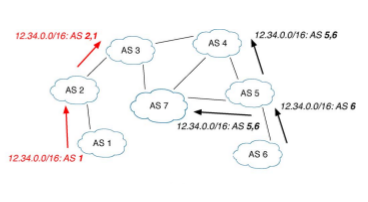
\includegraphics[scale=1]{pathlength1.png}
			\caption{Prefix hijacking by shorter AS pathes}
			\label{shortpath}
		\end{figure}
		Figure \ref{shortpath} shows an example where both AS 1 and AS 6 advertise the prefix 12.34.0.0/16 but just AS 6 owns those prefixes. The autonomous systems 2 and 3 may believe the advertisements from AS 1 because of the shorter path length in comparison to AS 6.

		\paragraph{Deaggregation}
		Another possibility to hijack prefixes is to advertise more specific routes. That means that an IP router would rather prefer a route to a smaller subnet than to a big block of adresses. This behaviour is called \emph{deaggregation.} 
		
		%TODO In 1997  
		\begin{figure}[h]
			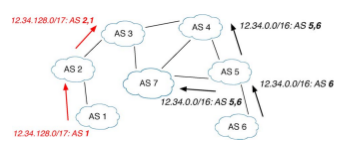
\includegraphics[scale=1]{deaggregation.png}
			\caption{Prefix hijacking by deaggregation}
			\label{deaggregation}
		\end{figure}
		An example of deaggreation is shown in \mbox{Figure \ref{deaggregation}}. Here all other autonomous systems will relay the traffic with destination 12.34.128.0/17 to AS 1, because it anounces a more specific prefix than AS 6 which advertises a larger block of IP addresses (12.34.0.0/16).
		
	       	\subsubsection{Attacks on TCP}
		BGP routers exchange information by utilizing the Transmission Control Protocll (TCP) to construct a realiable, connection-oriented channel between each other. 
		TCP already offers features like retransmission, error correction, congestion and flow control. 
		Since TCP itself does not offer a security mechanism that protects the messages confidentiality and integrity, those threats obviously exist for the communication between BGP routers. 
		In all described techniques we consider two BGP routers named Alice and Bob. The attacker, from now on called Malice, will try to compromise the normal operation and communication of those two routers.

		Possible attacks are eavesdropping on messages to learn routing information or reveal confidential buisness relationsships.
		Additionally, Man In The Middle attacks on TCP allow Malice to insert, modify and delete messages. 
		Also packets could be replayed to withdraw valid routes or re-install already withdrawn routes.
	
		Another way to affect BGP via TCP is a \emph{Denial-of-Service} attack, which will leave a BGP router unavailable to its users.
		It can be accomplished by the use of various techniques that will be described here briefly:
		\paragraph{TCP RST}
		A TCP connection can be closed by sending a TCP packet with either the FIN or RST flag set. 
		Malice could disrupt the conversation of Alice and Bob by sending a RST packet which will close the TCP connection between them. TCP has limited protection aka sequence numbers against this method. 

		\paragraph{SYN-Flood}
		The establishment of a TCP connection is initiated with the so called three-way handshake, a sequence of TCP messages with specific flags set. It starts with a SYN packet from Alice. Bob answers this SYN with a SYN-ACK. The handshake is completed by Alice, acknowledging the SYN-ACK from Bob with an ACK.
		Since Bob has to allocate resources when receiving a SYN from Alice, Malice could abuse this and exhaust the resources of Bob by sending alot of SYN packets without completing the handshake. This will make Bob unable to answer any further, real TCP connections. This can also lead to \emph{route flapping} which is described in the next paragraph.
		\paragraph{Route Flapping}
		Route flapping occurs when a router alternatly announces a route as unavailable and available again. When Malice achieves that Bob is no longer availablewith help of a DoS attack, Bobs neighbours will withdraw all routes they learned from Bob. Coming back online, Bob will advertise the routes again to all his neighbours.
		This behaviour results in a high use of network bandwith in addition to the DoS attack. 

		\subsubsection{Attack on the routing policy} 
		
		These attacks aim to influence the routers decision which route out of a set of routes should be anounced for a specific prefix. This decision depends on the attribute values in UPDATE messages. Routing policies of an AS determine on how those values are chosen. The following attributes are considered when chosing a route:
		\begin{itemize}
			\item The local preference attribute is used to prefer specific policies like contracts with customers over shortest-path routing.
			\item The AS path length is considered when multiple routes have the same local preference. The shorter path is chosen.
			\item The Origin type determines where the route was learned from. This could be from inside or outside the AS or from another type of source.
			\item It can occur that two huge 
		\end{itemize}
		Exploiting as path length and MED to manipulate route selection by an AS



       \section{BGP security today}
	target:	byzantine robustness
	Currently used: Protection of the TCP connection and defensive filtering
	
%Cryptographig techniques: 
%	Pairwise keying
%	Cryptographic hash functions
%	MACs
%	Diffie-Hellmann%	PKI
%	Certificates	


	\subsection{Protection of a BGP Session between routers}
	2 goals: Protecting TCP and BGP session itself
		Proposed solutions:
			MD5 integrity: Utilize TCP extension that uses a MAC based on MD5
					-> Protects integrity and prevents replay attacks

			Session and Message Protection:
				5 Proposed countermeasures:
					Adding sequence numbers
					Encryption of all BGP data between peers (shared secret)
					
					Adding UPDATE sequence numbers/timestamp
					New path attribute: PREDECESSOR: identification of last AS before destination
					digital signatures of all UPDATE fields
				Disadvantages: BGP needs to be altered
					       Based on shared secrets => hard to manage
			Hop Integrity Protocols:
				Peers can detect modification or replay attacks	
				Implemented by using sequence numbers, MACs and a PKI to refresh key

			Generalized TTL Security Mechanism
				Utilizing IP TTL to discard every packet with TTL < MAX-1. 
				
				=> Weakly defends against remote attacker, but not against malicious information coming from adjacent peers
				=> Also, useless in multihop environments
				
			IPsec
				Use IPsec to secure BGP at IP layer 
				IKE for key management, AH and ESP for packet level security
				Typically used to secure messages between peers
				Provides: authenticy, integrity, replay prevention, confidentality, DOS prevention
			


       \subsection{Defensive Filtering of suspicious BGP anouncments}
	Goal: Filter bad and potential malicious announcmentce 
	Usually ingress and egress filtering based on route policies like:
			prefixes with special uses
			bogons/martians (advertisements of adress blocks and AS numbers with no matching allocation data)
				=> filtering using an updated list of bogons
			filter out private AS numbers
			too long AS-Pathes
			routes to small soubnets (snm > 24) 
			hard limit of announcments by a neighbour 
			filtering by customer policies
				

       \subsection{Routing Registries}
		Approach: Beeing able to have a global view on correct routes makes it easy to detect attacks
		This could be achieved by creaint a routing registry that stores the following attributes:
			prefix ownership
			Connectivity between ASes
			routing policies
			
		Problems: 
			Such a registry has to be accurate, complete and secure
			Routing information sometimes intendet not to be public available
			Full trust on registry (SPoF)
			Information may become outdated due to lazy update policies
       		
       
       
       %Securing router managment
       %	Protection against physical attacks, SNMP attacks, DoS Attacks
       %       => Basic security, won't mention
       		
       			
	All of those described solutions are not sufficient for the protection of BGP

       \section{BGP Security Solutions}

       Multiple complete security architectures have been proposed to 
       \subsection{S-BGP}
			Validates Path attributes in BGP-Update by utilizing a PKI
			Data like adress ownership, peer AS identiy, control messages, policy attributes and path vectors can be digitally signed and verified
			The ownership of a prefix is checked by an out of band mechanism called Adress attestations by the validation of a delegation chain (similar to x509 PKI)
			Route attestations happen within BGP by appending a new attribute to the BGP UPDATE mesage. Each AS in the AS path signs prior signatures.
			Problems: 
				Huge amount of data that needs to be processed and number of possible signers makes this solution computational expensive
				
	\section{Conclusion}				

	
	\section{Literature}

\end{document}
